\documentclass[10pt]{beamer}
\usepackage[utf8x]{inputenc}
\usepackage{hyperref}
\usepackage{fontawesome}
\usepackage{graphicx}
\usepackage[english,ngerman]{babel}
% ------------------------------------------------------------------------------
% Use the beautiful metropolis beamer template
% ------------------------------------------------------------------------------
\usepackage[T1]{fontenc}
\usepackage{fontawesome}
\usepackage{FiraSans} 
\mode<presentation>
{
  \usetheme[progressbar=foot,numbering=fraction,background=light]{metropolis} 
  \usecolortheme{default} % or try albatross, beaver, crane, ...
  \usefonttheme{default}  % or try serif, structurebold, ...
  \setbeamertemplate{navigation symbols}{}
  \setbeamertemplate{caption}[numbered]
  %\setbeamertemplate{frame footer}{My custom footer}
} 

% ------------------------------------------------------------------------------
% beamer doesn't have texttt defined, but I usually want it anyway
% ------------------------------------------------------------------------------
\let\textttorig\texttt
\renewcommand<>{\texttt}[1]{%
  \only#2{\textttorig{#1}}%
}

% ------------------------------------------------------------------------------
% minted
% ------------------------------------------------------------------------------
\usepackage{minted}


% ------------------------------------------------------------------------------
% tcolorbox / tcblisting
% ------------------------------------------------------------------------------
\usepackage{xcolor}
\definecolor{codecolor}{HTML}{FFC300}


\usepackage{tcolorbox}
\tcbuselibrary{most,listingsutf8,minted}

\tcbset{tcbox width=auto,left=1mm,top=1mm,bottom=1mm,
right=1mm,boxsep=1mm,middle=1pt}

\newtcblisting{myr}[1]{colback=codecolor!5,colframe=codecolor!80!black,listing only, 
minted options={numbers=left, style=tcblatex,fontsize=\tiny,breaklines,autogobble,linenos,numbersep=3mm},
left=5mm,enhanced,
title=#1, fonttitle=\bfseries,
listing engine=minted,minted language=r}


% ------------------------------------------------------------------------------
% Listings
% ------------------------------------------------------------------------------
\definecolor{mygreen}{HTML}{37980D}
\definecolor{myblue}{HTML}{0D089F}
\definecolor{myred}{HTML}{98290D}

\usepackage{listings}

% the following is optional to configure custom highlighting
\lstdefinelanguage{XML}
{
  morestring=[b]",
  morecomment=[s]{<!--}{-->},
  morestring=[s]{>}{<},
  morekeywords={ref,xmlns,version,type,canonicalRef,metr,real,target}% list your attributes here
}

\lstdefinestyle{myxml}{
language=XML,
showspaces=false,
showtabs=false,
basicstyle=\ttfamily,
columns=fullflexible,
breaklines=true,
showstringspaces=false,
breakatwhitespace=true,
escapeinside={(*@}{@*)},
basicstyle=\color{mygreen}\ttfamily,%\footnotesize,
stringstyle=\color{myred},
commentstyle=\color{myblue}\upshape,
keywordstyle=\color{myblue}\bfseries,
}


% ------------------------------------------------------------------------------
% The Document
% ------------------------------------------------------------------------------
\title{Workshop: Datenbrille}
\author{Georg Jehle}
\date{Juni 2020}

\begin{document}

\maketitle

%\section{Introduction}
\begin{frame}[fragile]{Übersicht}
Teil 1: Datenbrillen und Linsenoptik\\
Teil 2: Microcontroller und Arduino \\
Teil 3: Programmieren
\end{frame}

\begin{frame}{Datenbrillen}
\textbf{Idee hinter Datenbrillen}\\[2mm]
\begin{itemize}
	\item Computergestützte Erweiterung des realen Sichtfelds (\emph{augmented reality})
	\item Zentrales Element: Überblendung von mehreren Bildprojektionen \\
	Bsp.: Sichtfeld überblendet mit Meta-Informationen
	\item Zusätzliche Informationen werden genutzt als Unterstützung bei bestimmten Arbeiten, als Orientierungshilfe, Live-Analyse, ...
	\item Technische Umsetzung: viele Varianten 
\end{itemize}
\end{frame}


\begin{frame}[fragile]{Datenbrillen: Beispiele i}
\textbf{Head-Up Display} \footnotemark\\[2mm]
\begin{minipage}{6.5cm}
	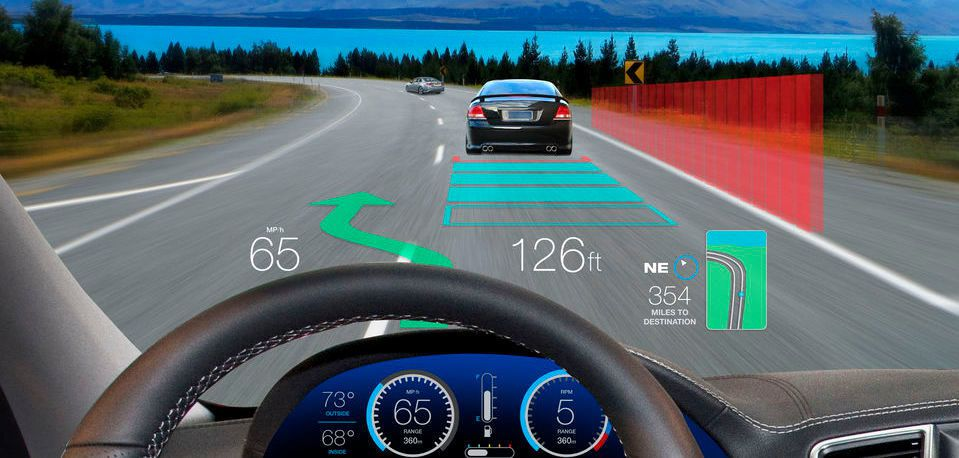
\includegraphics[height=3cm]{Bilder/Head-up-display.jpg}
\end{minipage}\hspace*{0.2cm}
\begin{minipage}{3cm}
	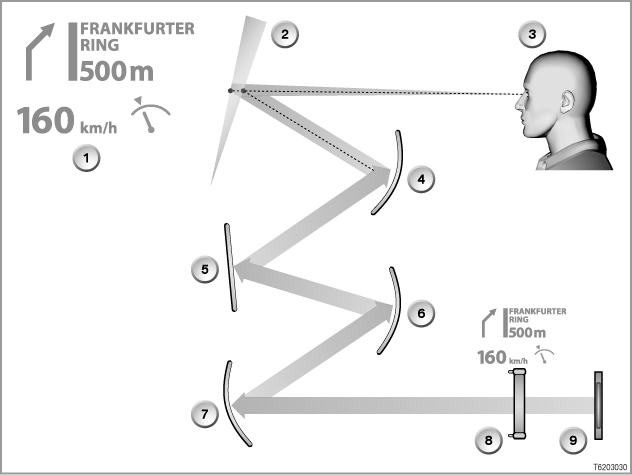
\includegraphics[height=3cm]{Bilder/Headupdisplay_funktion.png}
\end{minipage}\\
\begin{itemize}
	\item Licht des Displays wird über ein Spiegelsystem auf die Windschutzscheibe projiziert und ist als Reflexion erkennbar
	\item An einer bestimmten Position der Fahreraugen ist alles sichtbar und scharf
	\item Meta-Informationen kommen aus Fahrdiagnostik und Internet
\end{itemize}

\footnotetext[1]{\url{next-mobility.news}, 28.6.2020}
\end{frame}

\begin{frame}[fragile]{Datenbrillen: Beispiele ii}
\textbf{Google-Brille} \footnotemark \\[2mm]
\begin{minipage}{5cm}
	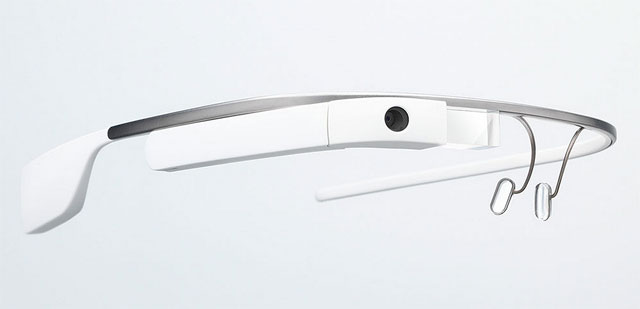
\includegraphics[height=2.5cm]{Bilder/google-brille-2.jpg}
\end{minipage}\hspace*{0.2cm}
\begin{minipage}{5cm}
	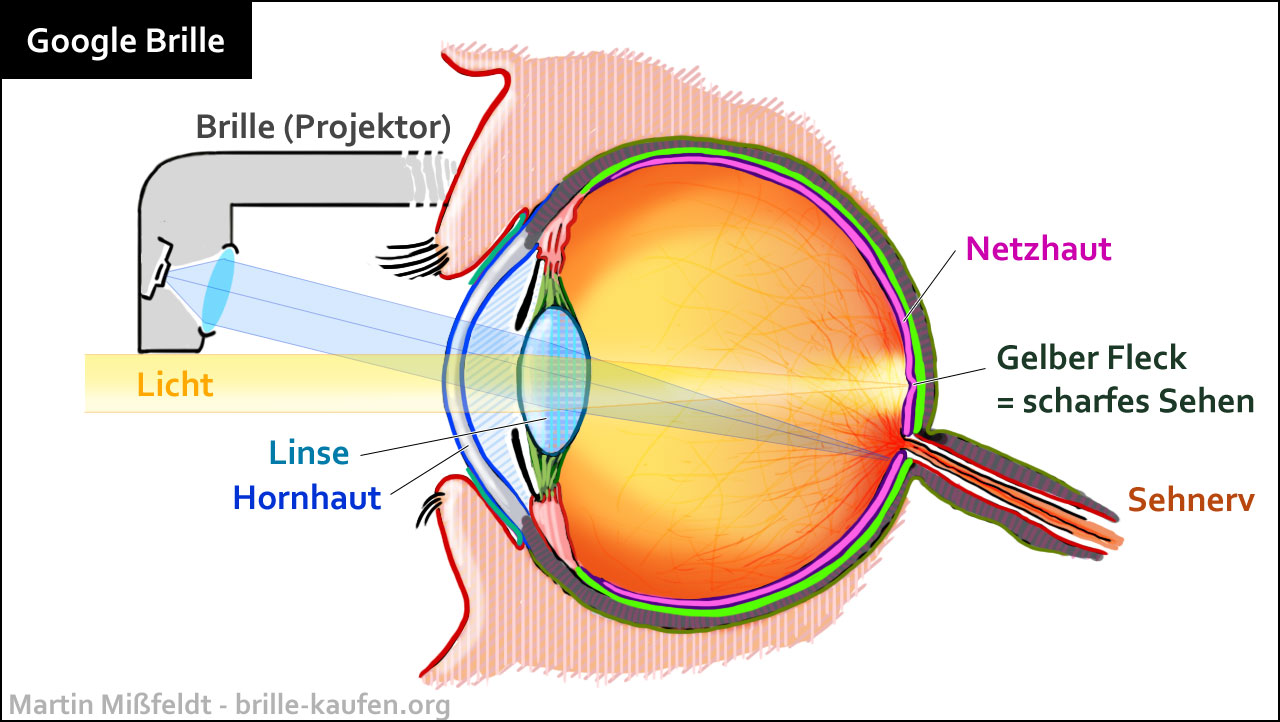
\includegraphics[height=2.5cm]{Bilder/google-brille-funktionsweise.jpg}
\end{minipage}\\
\begin{itemize}
	\item Licht wird direkt auf die Netzhaut projiziert 
	\item Anwender kann auf beliebige Stelle in Umgebung schauen, dann ist das Bild der Brille am Rand des Sichtfelds
	\item Datenbrille ist mit Internet verbunden
\end{itemize}
\footnotetext[2]{\url{notebookcheck.de}, 28.6.2020}
\end{frame}

\begin{frame}[fragile]{Datenbrillen: Beispiele iii}
\textbf{Datenbrille für Montagetechniker} \footnotemark\\[2mm]
\begin{minipage}{6.5cm}
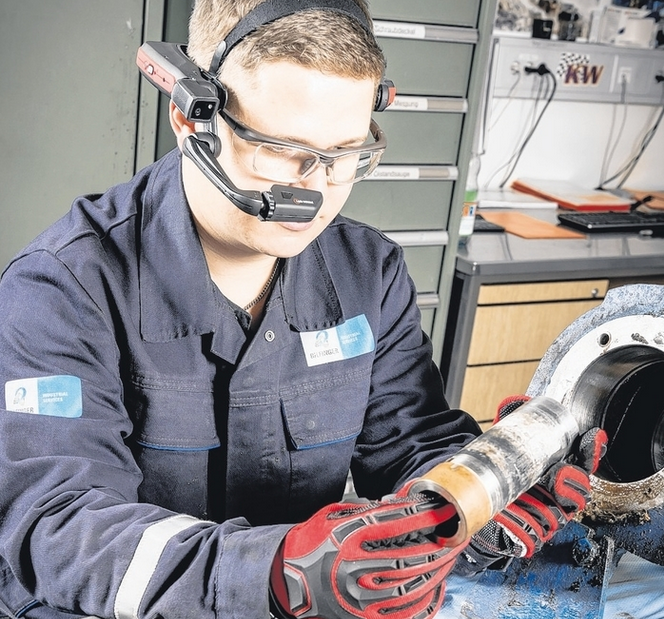
\includegraphics[height=3.5cm]{Bilder/Datenbrille_VDI_Techniker.png}
\end{minipage}\hspace*{0.2cm}
\begin{minipage}{3cm}
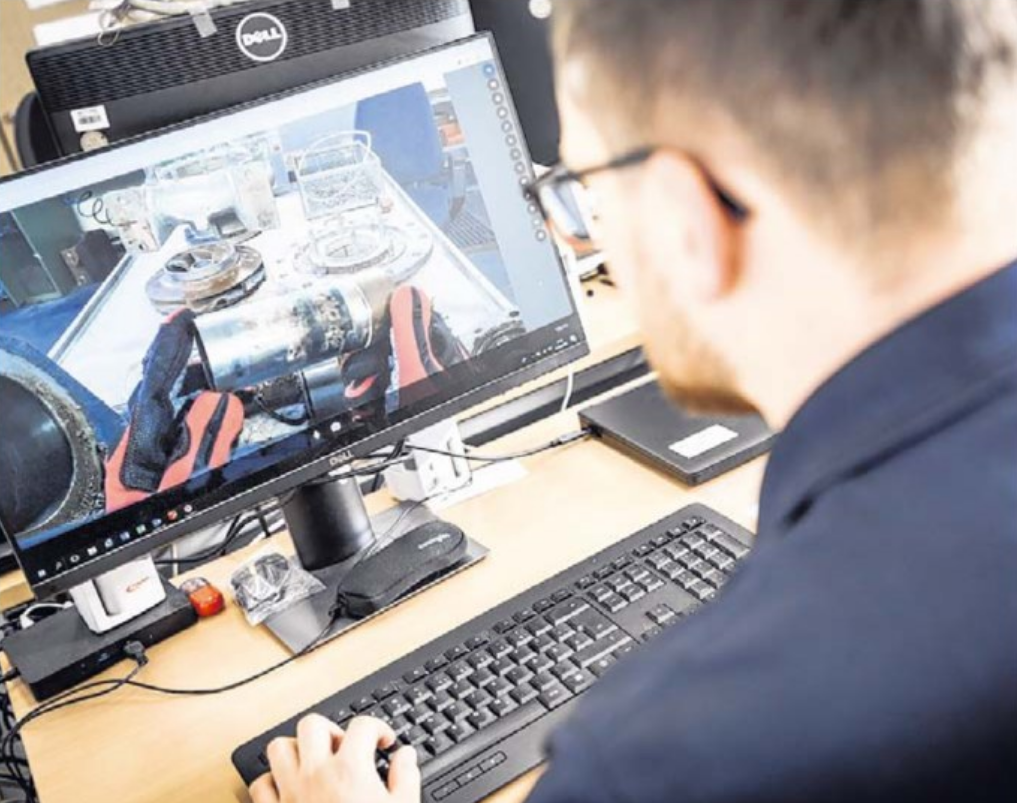
\includegraphics[height=3.5cm]{Bilder/Datenbrille_VDI_Ueberwachung.png}
\end{minipage}\\
\begin{itemize}
	\item Zusätzliche Kamera zur Übertragung des Sichtfelds 
	\item Ziel: Kontrolle (Fehlervermeidung)
	\item Kommunikation über Bild und Audio
\end{itemize}
\footnotetext[3]{\url{vdi-nachrichten.de}, 28.6.2020}
\end{frame}


\begin{frame}[fragile]{Datenbrille mit Fischertechnik}
\begin{minipage}{3cm}
	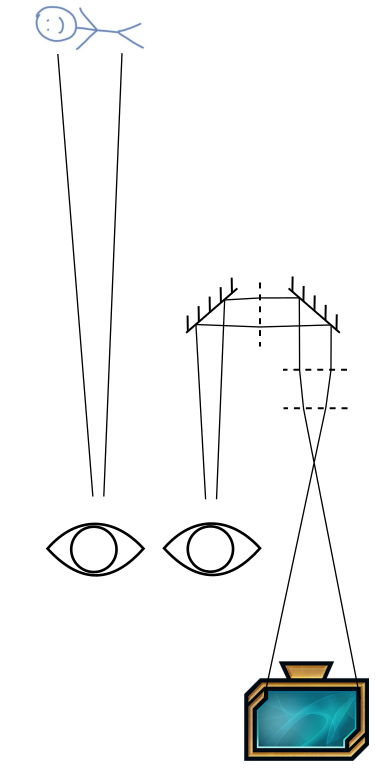
\includegraphics[height=5cm]{Bilder/Datenbrille_Strahlengang.png}
\end{minipage}\hspace*{0.5cm}
\begin{minipage}{7cm}
	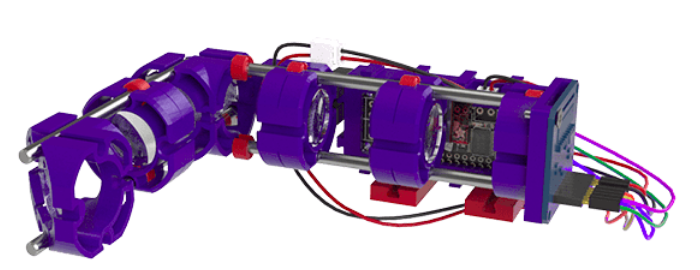
\includegraphics[width=7cm]{Bilder/datenbrille_bakaros.png}
\end{minipage}\\[2mm]
\begin{itemize}
	\item Ein Auge sieht Umgebung, das andere ein OLED-Display \\
	$\rightarrow$ Überblendung findet im Kopf statt
	\item Umlenkoptik auf OLED-Display durch drei plankonvexe Linsen und zwei Spiegel 
	\item Anzeige muss von uns programmiert werden
\end{itemize}
\end{frame}

\begin{frame}[fragile,allowframebreaks]{Linsenoptik}
\textbf{Lichtbrechung an einer Grenzfläche}\\[2mm]
\begin{minipage}{5cm}
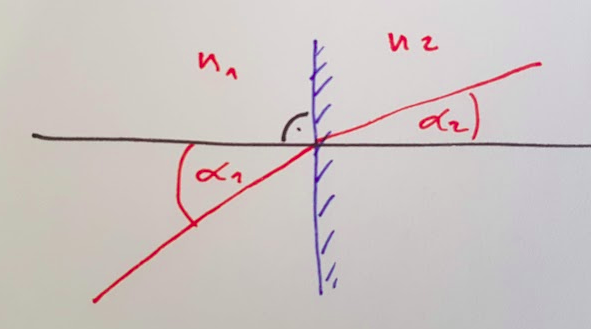
\includegraphics[width=\textwidth]{Bilder/Lichtbrechung.png}
\end{minipage}\hspace{2mm}
\begin{minipage}{5.5cm}
	Physikalische Eigenschaften von lichtdurchlässigen Medien beeinflussen die Lichtgeschwindigkeit. An Grenzflächen führt das zur Lichtbrechung.\\
	Beispiel: Person im Wasser
\end{minipage}\\[5mm]
\begin{minipage}{5cm}
\begin{itemize}
	\item Brechungsindex: $n_1$, $n_2$
	\item Lichtgeschwindigkeit: $c_1$, $c_2$
	\item Winkel: $\alpha_1$, $\alpha_2$
\end{itemize}
\end{minipage}\hspace{2mm}
\begin{minipage}{5.5cm}
\begin{align*}
	\frac{\sin(\alpha_1)}{\sin(\alpha_2)}=\frac{n_2}{n_1}=\frac{c_1}{c_2}
\end{align*}
\end{minipage}
\framebreak 

\textbf{Auswirkung auf Strahlengang durch konvexe Grenzfläche}\\[2mm]
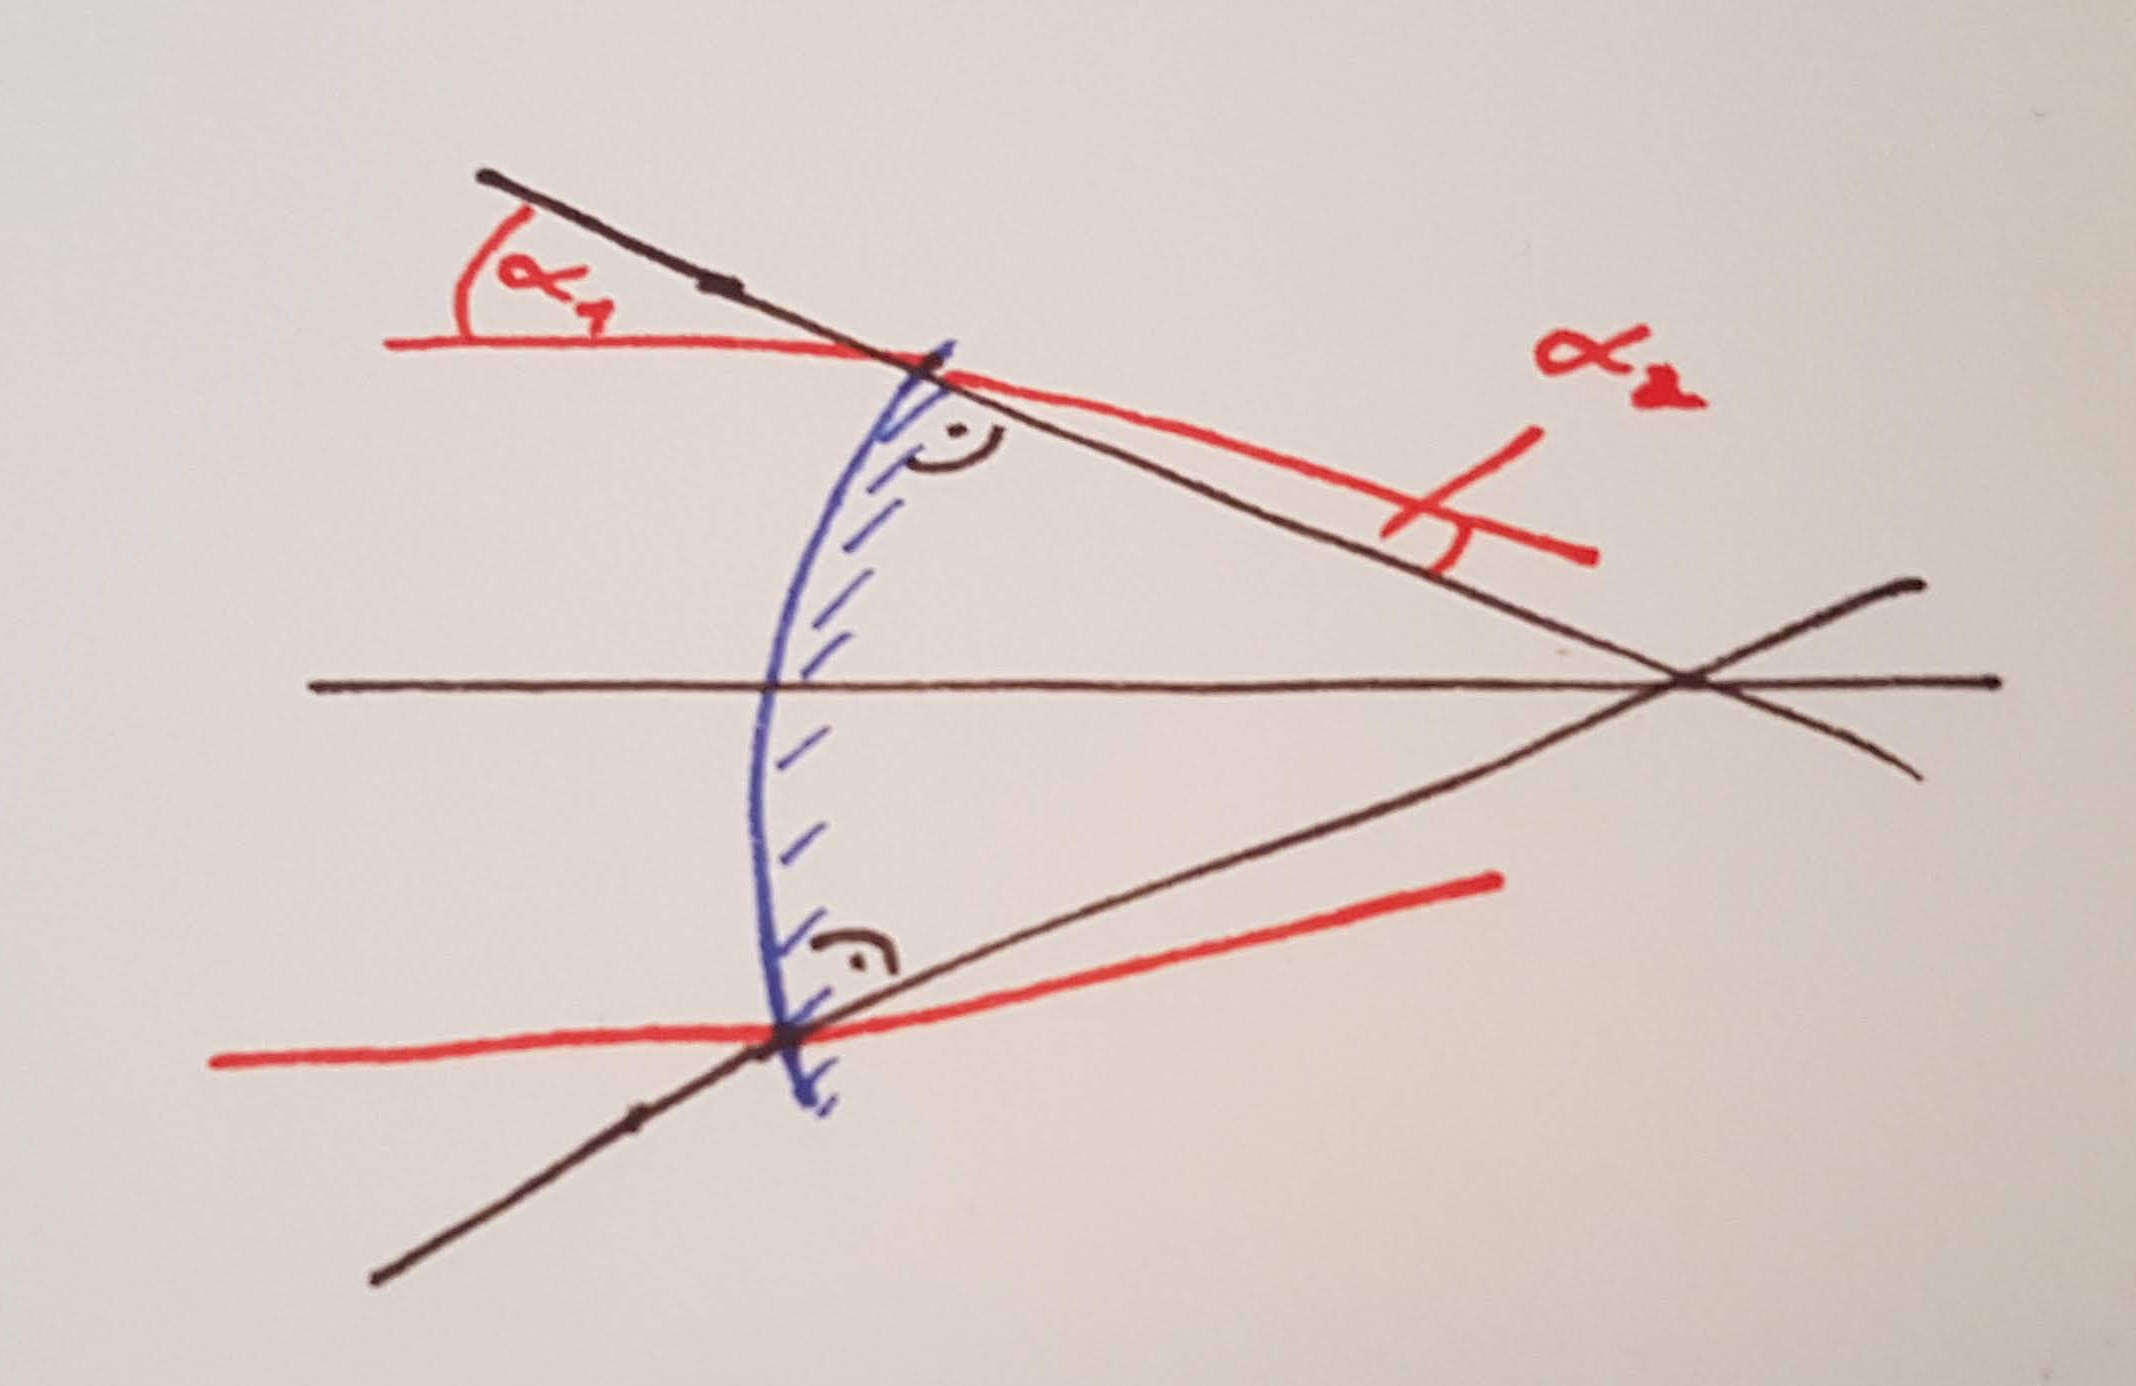
\includegraphics[width=6cm]{Bilder/Strahlengang1.jpg}\\[2mm]
Medium 1: Luft, Medium 2: Glas. $n_2>n_1$ $\rightarrow$ $\alpha_1>\alpha_2$\\
\textbf{Licht wird gesammelt }

\framebreak 
\textbf{Mehrere Linsen hintereinander} wie in unserer Datenbrille\\[2mm]
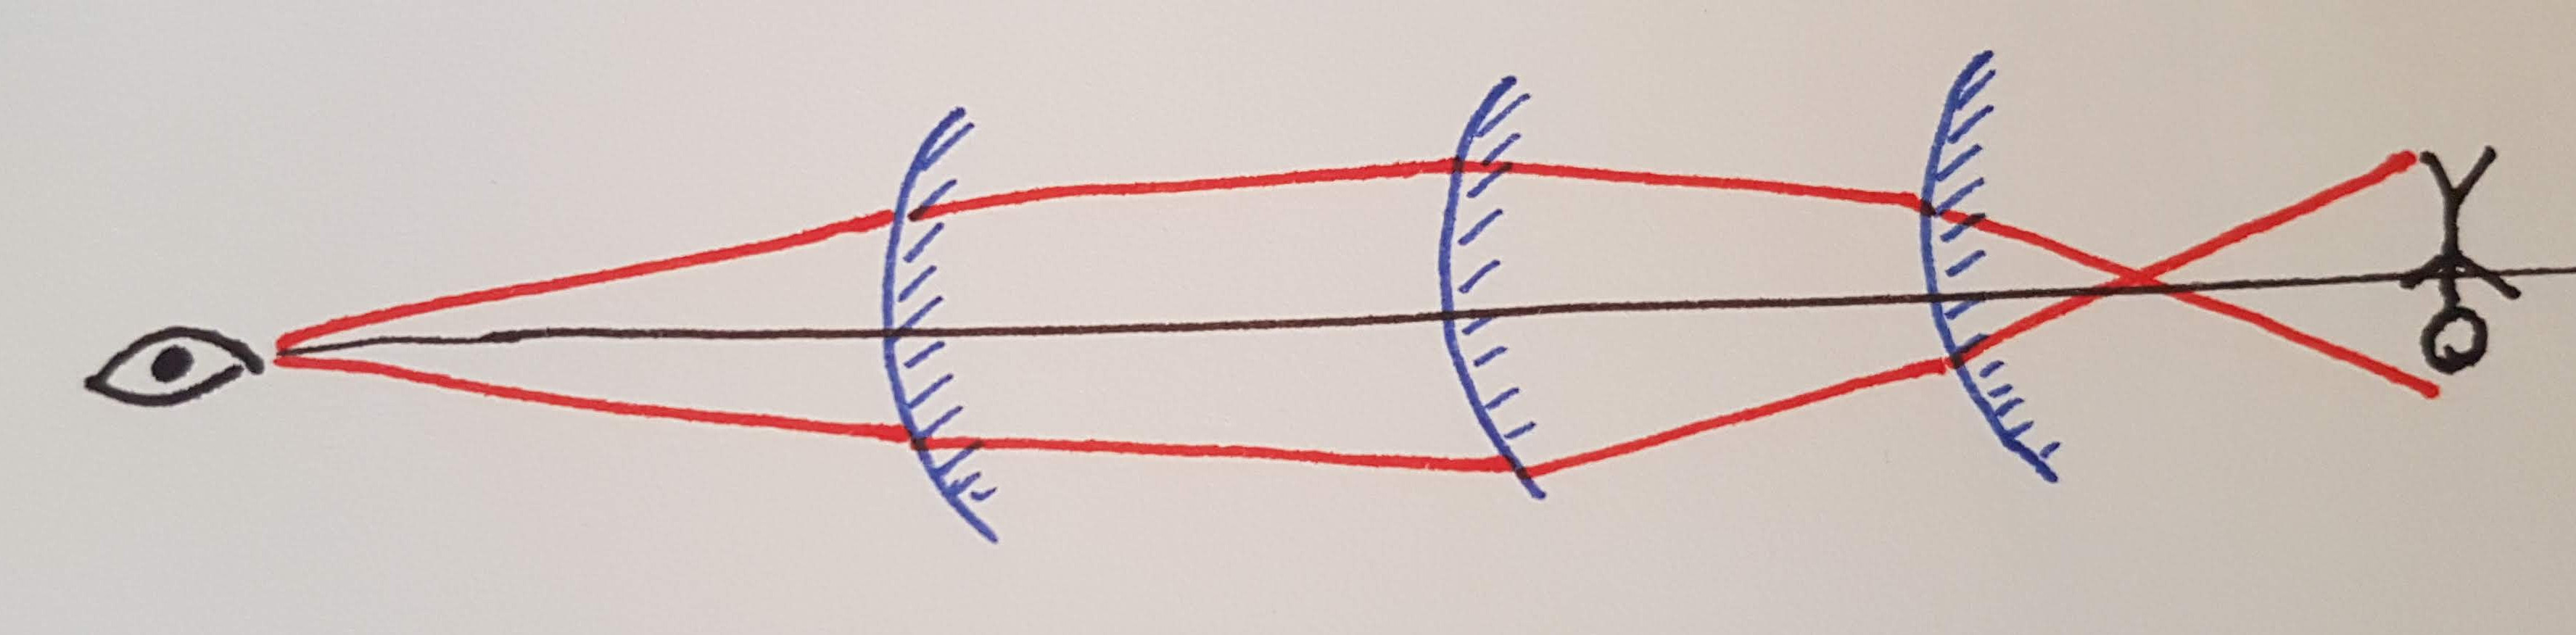
\includegraphics[width=8cm]{Bilder/Strahlengang2.jpg}\\[2mm]
Das Licht wird mehrmals gebündelt und dadurch nach der dritten Stufe in einem Fokus invertiert. Ein zweiter Fokus der Lichtstrahlen vom Display befindet sich im Auge, sodass das Bild hier scharf ist. Gleichzeitig kann eine Vergrößerung eingestellt werden. \\
\textbf{Parameter}: Abstand zwischen den Linsen

\framebreak 
\textbf{Spiegelung vs. Invertierung}\\[2mm]
Spiegelung: Lichtstrahlen werden an einer Ebene vertauscht \\
(z.B. rechts wird zu links, oben wird zu unten)\\[2mm]
Invertierung: Lichtstrahlen werden in einem Punkt (Fokus) vertauscht. Dann wird rechts oben zu links unten etc. 
\end{frame}

\begin{frame}[fragile,allowframebreaks]{Microcontroller und Arduino}
\textbf{Microcontroller:} Ein-Chip-Computersystem mit Peripherie- funktionen (Anschlüsse: USB, Ethernet, speziellere Anschlüsse). Einsatz heutzutage in fast allen technischen Geräten wie Drucker, Smartphone, Waschmaschine, ... Vorteile: sparsam (geringer Energieverbrauch im Vergleich mit PC), kostengünstig, wenig Bauraum. Nachteile: Leistung der Datenverarbeitung und Geschwindigkeit sind nicht so hoch. \\[2mm]
\textbf{Arduino:} Open-Source-Platform bestehend aus Hardware (Board, z.B. Uno oder Feather) und Software (Arduino IDE)\\[2mm]
\textbf{Download} der Installationsdatei der aktuellen Softwareversion: \url{https://www.arduino.cc/en/main/software} \\[2mm]
\textbf{Konfiguration:} Bibliotheken für OLED-Display (\texttt{adafruit\_ssd1306}) und Board (Feather ist in \texttt{arduino\_samd} enthalten) einbinden 


\framebreak
\textbf{Übersicht}\\[3mm]
\begin{minipage}{7cm}
	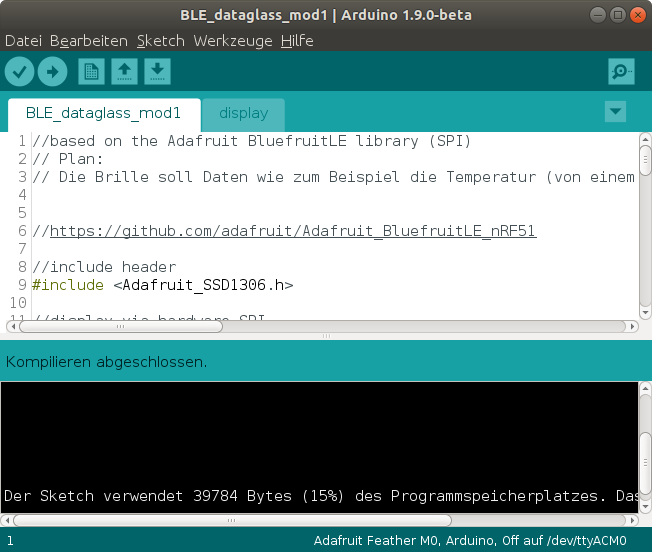
\includegraphics[height=6.1cm]{Bilder/Arduino.png}
\end{minipage}\hspace*{3mm}
\begin{minipage}{2cm}
Menüleiste\\[1mm]
Werkzeuge\\[10mm]
Textfeld (Programm)\\[10mm]
Ausgabefeld\\[12mm]
Schittstelle
\end{minipage}

\framebreak
\textbf{Konfigurieren:} Bibliothek \texttt{adafruit\_ssd1306} hinzufügen\\[3mm]
\begin{minipage}{7cm}
	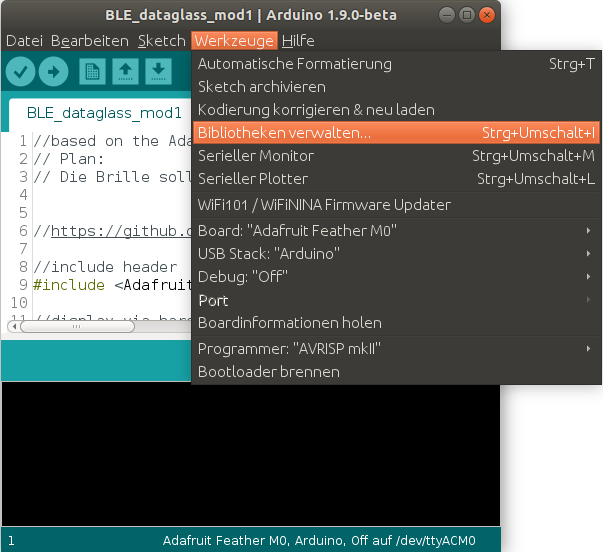
\includegraphics[height=6.1cm]{Bilder/Arduino_Bibliotheken1.png}
\end{minipage}\hspace*{3mm}
\begin{minipage}{2cm}
	Menüleiste\\[1mm]
	Werkzeuge\\[10mm]
	Textfeld (Programm)\\[10mm]
	Ausgabefeld\\[12mm]
	Schittstelle
\end{minipage}

\framebreak
\textbf{Konfigurieren:} Bibliothek \texttt{adafruit\_ssd1306} hinzufügen\\
Suche \texttt{adafruit\_ssd1306} $\rightarrow$ aktuelle Version installieren\\[3mm]
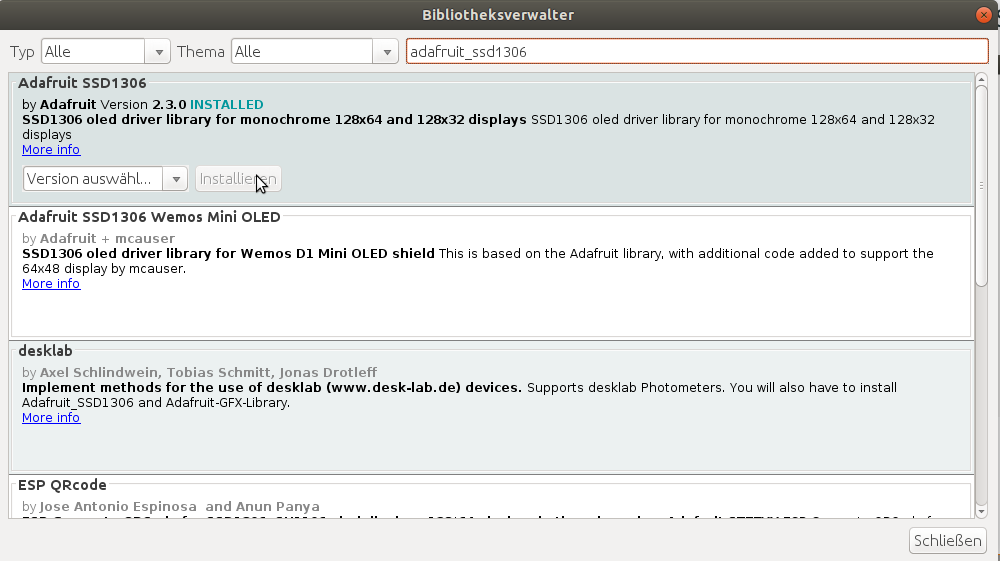
\includegraphics[height=5cm]{Bilder/Arduino_Bibliotheken2.png}

\framebreak
\textbf{Konfigurieren:} Bibliothek für Feather (\texttt{arduino\_samd}) hinzufügen\\
\begin{minipage}{7cm}
	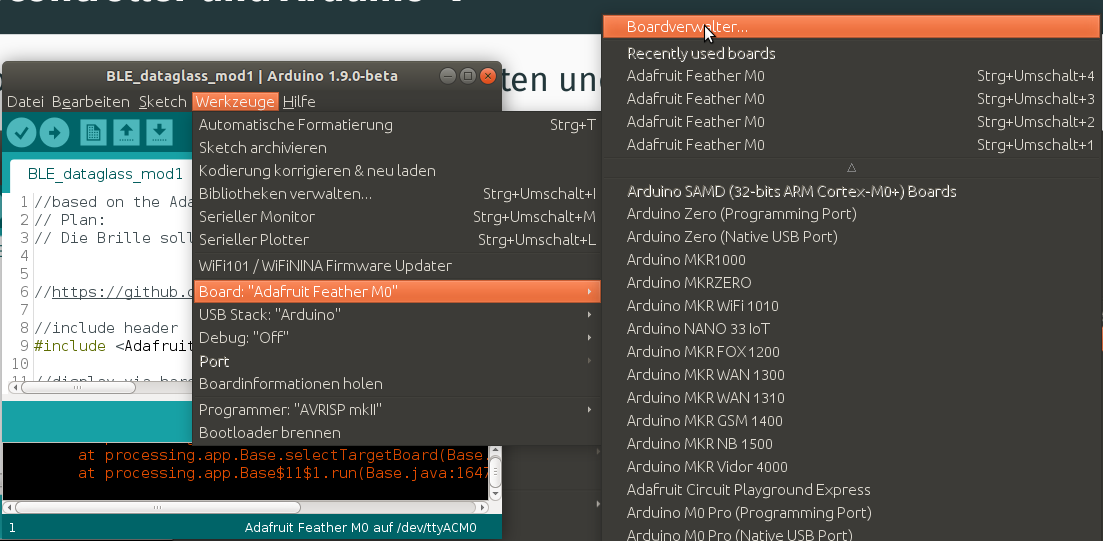
\includegraphics[height=5.5cm]{Bilder/Arduino_Boardverwalter1.png}
\end{minipage}\hspace*{3mm}


\framebreak
\textbf{Konfigurieren:} Bibliothek für Feather (\texttt{arduino\_samd}) hinzufügen\\
Suche \texttt{feather} oder \texttt{arduino\_samd} $\rightarrow$ aktuelle Version installieren\\[3mm]
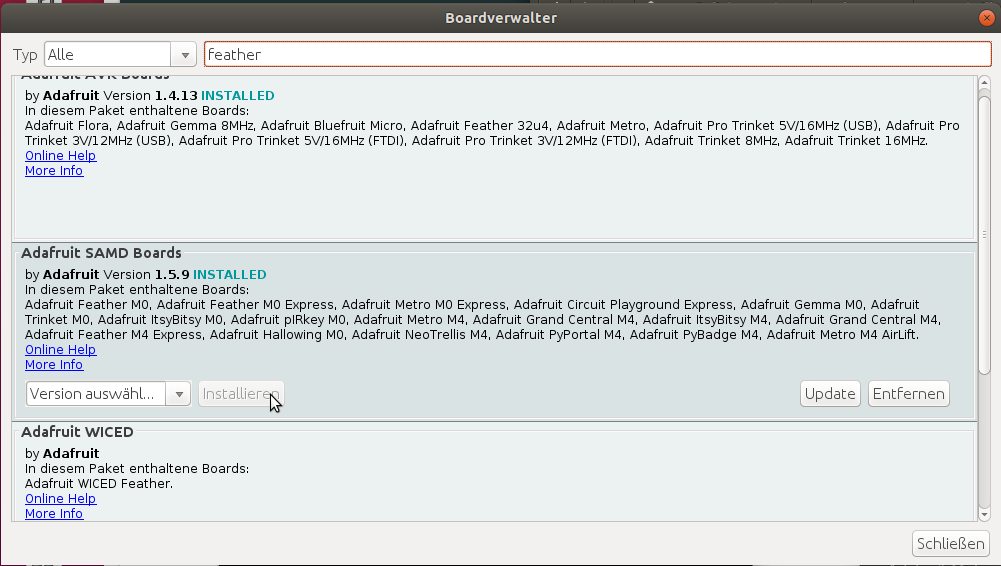
\includegraphics[height=5cm]{Bilder/Arduino_Boardverwalter2.png}



\framebreak
\textbf{Konfigurieren:} Richtiges Board einstellen\\[3mm]
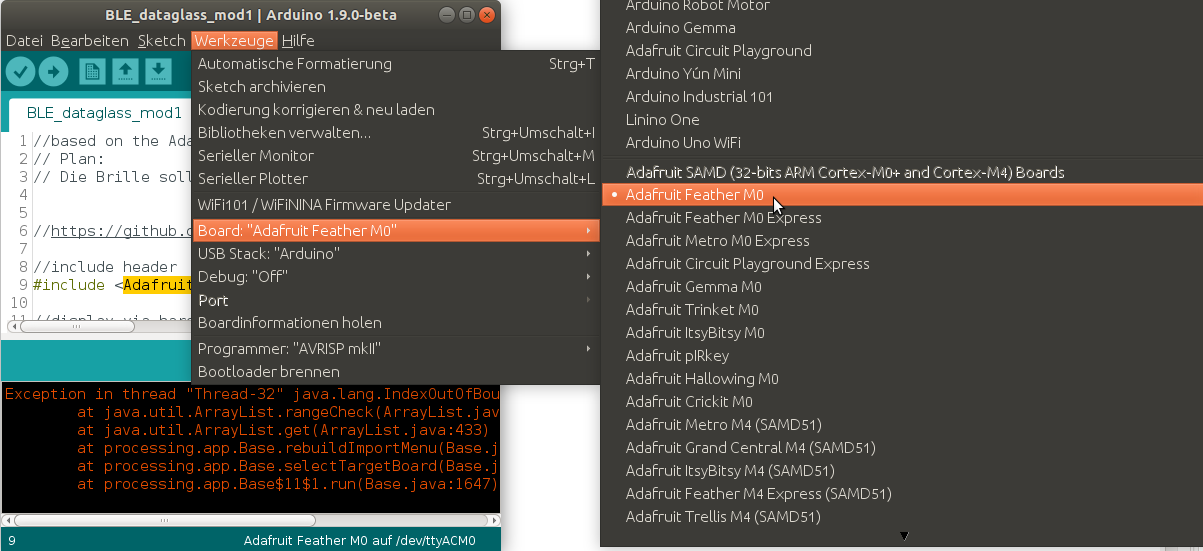
\includegraphics[height=5.5cm]{Bilder/Arduino_Bibliotheken3.png}\\
Spätestens danach steht als Schnittstelle ''Adafruit Feather M0''

\framebreak
\textbf{Code überprüfen:} (kompilieren, engl. \emph{to compile}: zusammensetzen) \\[3mm]
\begin{minipage}{6.1cm}
	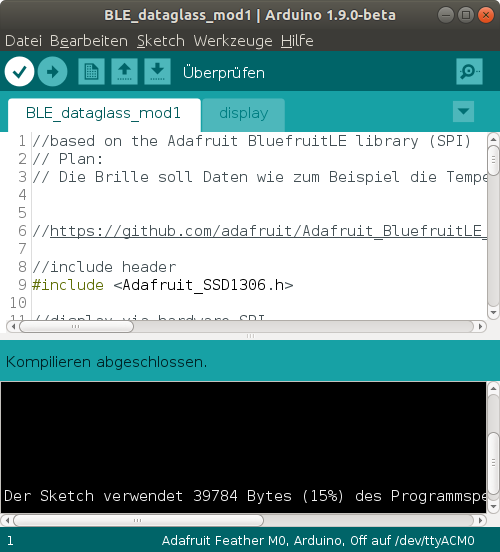
\includegraphics[height=6.1cm]{Bilder/Arduino_Ueberpruefen.png}
\end{minipage}\hspace*{3mm}
\begin{minipage}{4cm}
	Menüleiste\\[1mm]
	Werkzeuge\\[10mm]
	Textfeld (Programm)\\[10mm]
	Ausgabefeld\\[12mm]
	Schittstelle
\end{minipage}\\[0mm]
\textbf{Kompilieren}: Übersetzen des Programms in Maschinencode

\framebreak
\textbf{Fehler nach kompilieren:} \\[3mm]
\begin{minipage}{6.1cm}
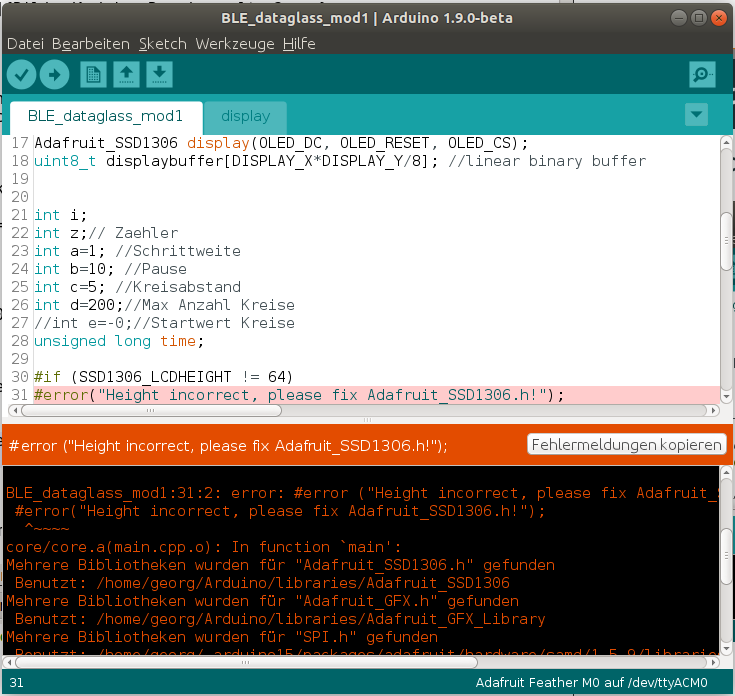
\includegraphics[height=6.1cm]{Bilder/Arduino_Fehler_Bildschirm.png}
\end{minipage}\hspace*{3mm}
\begin{minipage}{4cm}
\begin{itemize}
	\item Ausgabefeld: rote Meldungen
	\item Textfeld: Zeile 31 mit Fehler (Bug) rot markiert
	\item Hier: die Fehlermeldung wurde vom Programmierer eingebaut
\end{itemize}
\end{minipage}

\framebreak
\textbf{Fehler nach kompilieren:} Falsche Parameter in \texttt{adafruit\_ssd1306} \\[3mm]
\textbf{Problembehebung:} Öffne Sketchbook-Speicherort $\rightarrow$ \texttt{Arduino/} \texttt{libraries/Adafruit\_SSD1306/adafruit\_ssd1306.h}  und ersetze 
\metroset{block=fill}
\begin{exampleblock}{adafruit\_ssd1306.h}
%	\begin{verbatim}
\textcolor{red}{\texttt{//}}\verb|#define SSD1306_128_64 ///< DEPRECATED: ...|
\verb|#define SSD1306_128_32 ///< DEPRECATED: ...|
%	\end{verbatim}
\end{exampleblock}
durch
\begin{exampleblock}{adafruit\_ssd1306.h}
%	\begin{verbatim}
	\verb|#define SSD1306_128_64 ///< DEPRECATED: ...|
	\textcolor{mygreen}{\texttt{//}}\verb|#define SSD1306_128_32 ///< DEPRECATED: ...|
%	\end{verbatim}
\end{exampleblock}

\framebreak
\textbf{Hochladen:} Code kompilieren und auf Board überspielen\\[3mm]
\begin{minipage}{6.1cm}
	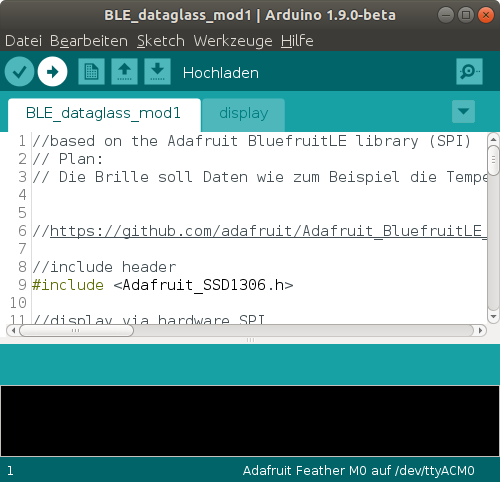
\includegraphics[height=6.1cm]{Bilder/Arduino_Hochladen.png}
\end{minipage}\hspace*{3mm}
\begin{minipage}{4cm}
	Menüleiste\\[1mm]
	Werkzeuge\\[10mm]
	Textfeld (Programm)\\[10mm]
	Ausgabefeld\\[12mm]
	Schittstelle
\end{minipage}
\end{frame}


\begin{frame}[fragile,allowframebreaks]{Code: Programmbausteine}

\metroset{block=fill}
\begin{exampleblock}{// Kommentar}
\begin{verbatim}
// Alles was in einer Zeile nach // folgt ist ein Kommen-
// tar. Ein Kommentar ist vom Kompilieren ausgenommen.
\end{verbatim}
\end{exampleblock}
\begin{exampleblock}{\# Compiler-Optionen}
	\begin{verbatim}
	// Compiler-Optionen erkennt man am vorgestellten # 
	// Bsp.: Bibliothek einbinden mit #include
	#include <adafruit_ssd1306.h> 
	// Bsp.: Variable OLED_DC auf Wert 5 setzen mit #define
	#define OLED_DC 5 
	\end{verbatim}
\end{exampleblock}
\begin{exampleblock}{Zuweisung}
\begin{verbatim}
// Deklaration der Ganzzahl i und Zuweisung des Werts
int i;  // "Es gibt die Variable i mit Datentyp int". 
i = 1;  // int hat den Wert 1 

// Beide Schritte in einer Zeile geht auch:
int i=1; 

// Am Ende einer Zuweisung muss ein ; stehen. Danach kommt 
// der nächste Befehl.
\end{verbatim}
\end{exampleblock}
\begin{exampleblock}{Objekte mit Methode ansprechen}
	\begin{verbatim}
	// Ein Objekt hat verschiedene Eigenschaften, die ange-
	// sprochen werden können
	
	// Syntax: Objekt.Methode(Argumente)
	
	display.begin(SSD1306_SWITCHCAPVCC); // Display starten
	display.setTextColor(WHITE); // Textfarbe auf weiß setzen
	
	\end{verbatim}
\end{exampleblock}
Weitere Methoden von display: 
\url{https://learn.adafruit.com/adafruit-gfx-graphics-library/graphics-primitives}
\end{frame}

\begin{frame}[fragile,allowframebreaks]{Text auf Display darstellen mit \texttt{display.print()}}
\metroset{block=fill}
\begin{exampleblock}{display.ino}
	\begin{verbatim}
	// Statischen Text auf Display ausgeben: 
	void Targeter() {
		display.setTextColor(WHITE);   // Textfarbe
		display.setCursor(30, 10);     // Cursorposition
		display.setTextSize(2);        // Textgröße
		display.setTextWrap(0);        // kein Zeilenumbruch
		display.clearDisplay();        // Display löschen
		display.print("Hallo Georg!"); // Textausgabe definieren
		display.display();             // Display aktualisieren
		delay(500);                    // Pause für 500 ms = 0.5 s
	}
	\end{verbatim}
\end{exampleblock}
\begin{exampleblock}{display.ino}
\begin{verbatim}
// statt display.print("Hallo Georg!") ab jetzt Folgendes:

display.print("Zeit=");  // statische Textausgabe
time = millis()/1000;    // Zeit in s ab Start berechnen 
display.print(time);     // Zeit auf Display werfen
\end{verbatim}
\end{exampleblock}
Achtung: die Variable \texttt{time} gibt es noch nicht. Sie muss zuerst in der Hauptfunktion deklariert werden: 
\begin{exampleblock}{BLE\_dataglass\_mod1.ino}
	\begin{verbatim}
	unsigned long time;
	\end{verbatim}
\end{exampleblock}
\end{frame}

\begin{frame}[fragile,allowframebreaks]{Kreis auf Display darstellen}
\metroset{block=fill}
\begin{exampleblock}{display.ino}
	\begin{verbatim}
	x = (display.width()-50)/2;
	y = (display.height()-50)/2;
	r = 50; 
	display.drawCircle(x, y, r, WHITE);
	\end{verbatim}
\end{exampleblock}
Deklarieren (\texttt{int}) nicht vergessen! 
\begin{exampleblock}{display.ino}
	\begin{verbatim}
	for (r_i = 0; r_i <= 10; r_i = r_i + 2) {
	    display.clearDisplay();
	    display.drawCircle(x, y, r_i, WHITE);
	    display.display();
	    delay(500);
	}
	\end{verbatim}
\end{exampleblock}
In einer \emph{for}-Schleife werde die beschriebenen Operationen für jeden Wert der Schleifenvariable r\_i ausgeführt. Der Startwert ist \texttt{0}, der Endwert \texttt{10}, die Schrittweite \texttt{2}. Also nimmt der Radius die Werte \texttt{r\_i=0,2,4,6,8,10} an, für den jeweils ein Kreis gezeichnet wird.  

\end{frame}

\begin{frame}[fragile]{Anregungen für Erweiterungen}
\begin{itemize}
	\item Lass die Kreise/Rechtecke von außen nach innen laufen! 
	\item Lass den Mittelpunkt der Kreise wandern! 
	\item Recherchiere im Internet, welche weiteren geometrischen Elemente darstellbar sind, und teste sie! 
\end{itemize}
\end{frame}

\end{document}
